\section{Experiments}\label{sec:experiments}

In this section we describe the results of experiments comparing
the run time of \Sparrow\ with those of two leading implementations of
boosted trees: XGBoost and LightGBM.

\begin{table}[]
\centering
\label{table-exp}
\begin{tabular}{|l|l|c|c|}
\hline
Algorithm            & Instance & Instance Memory \iffalse{& Memory Usage}\fi & Training (minutes)  \\ \hline
XGBoost, in-memory   & \texttt{x1e.xlarge}    & 122 GB          \iffalse{& 105.6 GB}\fi          & 414.6                                  \\
XGBoost, off-memory  & \texttt{r3.xlarge}     & 30.5 GB         \iffalse{& 3.9 GB}\fi            & 1566.1                                  \\
LightGBM, in-memory  & \texttt{x1e.xlarge}    & 122 GB          \iffalse{& 41.6 GB}\fi           & 341.6                                  \\
LightGBM, off-memory & \texttt{r3.xlarge}     & 30.5 GB         \iffalse{& 16.8 GB}\fi           & 449.7                                  \\
\multirow{2}{*}{TMSN, sample 10\%}    & \multirow{2}{*}{\texttt{c3.xlarge}}     & \multirow{2}{*}{7.5 GB}          \iffalse{& \multirow{2}{*}{3.4 GB}}\fi            & 57.4 (1 worker)      \\
                     &                        &                                    & 17.7 (10 workers) \\ \hline
\end{tabular}
\vspace{0.2cm}
\caption{Experiments on the Splice Site Detection Task}
\end{table}

\paragraph{Setup}
We use a large dataset that was used in other studies of large scale
learning on detecting human acceptor splice site~\cite{sonnenburg_coffin:_2010, agarwal_reliable_2014}.
The learning task is binary classification.
We use the same training dataset of 50\,M samples as in the other work,
and validate the model on the testing data set of 4.6\,M samples.
The training dataset on disk takes over 27\,GB in size.

As the code is not fully developed yet, we restrict our trees to one
level so-called ``decision stumps''. We plan to perform comparisons
using multi-level trees and more than two labels. We expect similar
runtime performance there. To generate comparable models,
we also train decision stumps in XGBoost and LightGBM
(by setting the maximum tree depth to 1).

Both XGBoost and LightGBM are highly optimized, and support multiple
tree construction algorithms.
For XGBoost, we selected approximate greedy algorithm for the efficiency purpose.
LightGBM supports using sampling in the training,
which they called \textit{Gradient-based One-Side Sampling (GOSS)}.
GOSS keeps a fixed percentage of examples with large gradients,
and then randomly sample from remaining examples with small gradients.
We selected GOSS as the tree construction algorithm for LightGBM.

All algorithms in comparison optimize the exponential loss as defined in AdaBoost.
We also evaluated the final model by calculating its area under precision-recall
curve (AUPRC) on the testing dataset.

Finally, the experiments are all conducted on EC2 instances from Amazon Web Services.
Since XGBoost requires 106\,GB memory space for training this dataset in memory,
we used instances with 120\,GB memory for such setting.
Detailed description of the setup is listed in Table~\ref{table-exp}.

\paragraph{Evaluation}
Performance of each of the algorithm in terms of
the exponential loss as a function of time on the testing dataset is given in
Figure~\ref{fig:loss}. Observe that all algorithms achieve similar
final loss, but it takes them different amount of time to reach that
final loss. We summarize these differences in Table~\ref{table-exp} by
using the convergence time to an almost optimal loss of
$0.061$. Observe  XGBoost off-memory is about 27
times slower than a single \Sparrow\ worker which is also off-memory. That
time improves by another factor of 3.2 by using 10 machines instead of 1.

In Figure~\ref{fig:auprc} we perform the comparison in terms of
AUPRC. The results are similar in terms of speed. However, in this
case XGBoost and LightGBM ultimately achieve a slightly better
AUPRC. This is baffling, because all algorithms work by minimizing
exponential loss.

\begin{figure}[t]
    \centering
    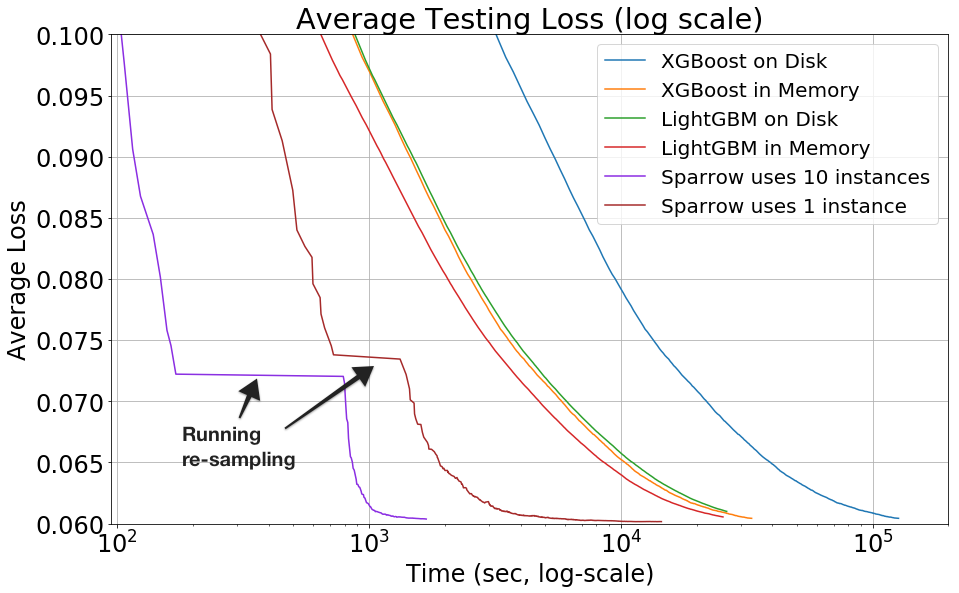
\includegraphics[width=0.5\textwidth]{splice-loss.png}
    \caption{Comparing the average loss on the testing data using \Sparrow, XGBoost, and LightGBM, lower is better.
        The period of time that the loss is constant for \Sparrow\ is when the algorithm is generating a new sample set.}~\label{fig:loss}
\end{figure}



\begin{figure}[t]
    \centering
    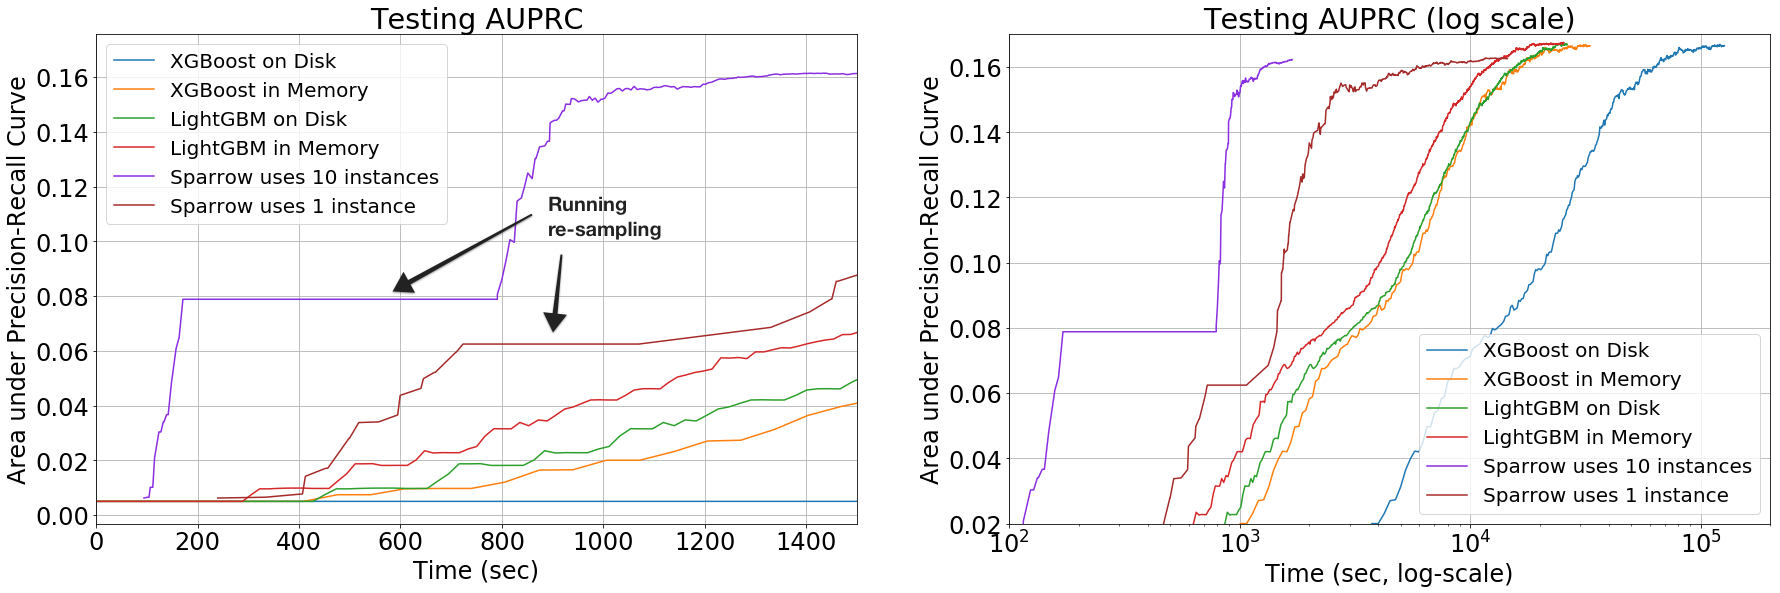
\includegraphics[width=0.5\textwidth]{splice-auprc.png}
    \caption{Comparing the area under the precision-recall curve (AUPRC) on the testing data
    using \Sparrow, XGBoost, and LightGBM, higher is better.
    (left) Normal scale, clipped on right.
    (right) Log scale, clipped on left.
    The period of time that the AUPRC is constant for \Sparrow\ is when the algorithm is generating a new sample set.}~\label{fig:auprc}
\end{figure}


\paragraph{Conclusions}
While the results are exciting plenty of work remains. We plan to
extend the algorithm to boosting full trees as well as other types of
classifiers.
In addition, we observe that run time is now dominated by the time it
takes to create new samples, we have some ideas for how to
significantly reduce the sampling time.





\iffalse

\begin{table}[h]
\centering
\caption{Dataset used in the experiments}\label{tab:dataset}
\begin{tabular}{|l|ccccc|}
\cline{1-6}
Dataset         & Fraction    & \# Features & Training    &  Training  & Testing     \\
                & of rare set &             & \#exmaples  &  data size & \#examples  \\ \cline{1-6}
Human splicing  & 0.3\%       & 141         & 50,000,000  &            & 4627840     \\ \cline{1-6}
Higgs Boson     &             & 28          & 10,000,000  &            & 1,000,000   \\ \cline{1-6}
\end{tabular}
\end{table}

\subsection{Comparison to XGBoost and LightGBM}


A table comparing the amount of time it takes for each to converge.

\subsection{Effect of Early Stopping}
Plot number of examples (as fraction of all training examples) scanned until stopping rule fires and  tree is added (single machine)

\subsection{Effect of selective Sampling}
Give plots of training and test loss with no resampling, one resampling, two resampling

\subsection{Effect of parallelization}
Compare running on one machine and running on 10 (Do another resampling at around 0.16 prc)



\fi
